\documentclass{article}
\usepackage[paperwidth=90in,paperheight=42in,margin=0in]{geometry}
\usepackage{tikz}
\usepackage{graphicx}
\usepackage{xcolor}
\usepackage{fontspec}
\setmainfont{Helvetica}
\setsansfont{Helvetica}
\definecolor{poster050505}{HTML}{050505}
\definecolor{poster111111}{HTML}{111111}
\definecolor{poster242424}{HTML}{242424}
\definecolor{poster4a4a4a}{HTML}{4a4a4a}
\definecolor{poster8a8a8a}{HTML}{8a8a8a}
\definecolor{posterf1f1f1}{HTML}{f1f1f1}
\definecolor{posterfafafa}{HTML}{fafafa}
\definecolor{posterffffff}{HTML}{ffffff}
\pagestyle{empty}
\begin{document}
\begin{tikzpicture}[x=1in,y=1in]
\path[fill=posterffffff, draw=none] (0.000,42.000) rectangle (90.000,0.000);
\path[fill=poster050505, draw=none, rounded corners=0.045in] (1.200,41.300) rectangle (4.650,37.850);
\node[anchor=north west, text width=2.950in, align=center, inner sep=0pt] at (1.450,40.650) {\color{posterffffff}\bfseries \fontsize{1.200in}{1.440in}\selectfont \centering \spaceskip=0.32em plus 0.10em minus 0.06em NYU\par};
\node[anchor=north west, text width=11.000in, align=left, inner sep=0pt] at (5.350,40.980) {\color{poster050505}\bfseries \fontsize{0.780in}{0.936in}\selectfont \raggedright \spaceskip=0.32em plus 0.10em minus 0.06em New York University\par};
\node[anchor=north west, text width=11.000in, align=left, inner sep=0pt] at (5.350,39.950) {\color{poster4a4a4a}\fontsize{0.560in}{0.672in}\selectfont \raggedright \spaceskip=0.32em plus 0.10em minus 0.06em Department of Psychology\par};
\node[anchor=north west, text width=11.000in, align=left, inner sep=0pt] at (5.350,39.250) {\color{poster4a4a4a}\fontsize{0.560in}{0.672in}\selectfont \raggedright \spaceskip=0.32em plus 0.10em minus 0.06em Center for Neural Science\par};
\node[anchor=north west, text width=52.000in, align=center, inner sep=0pt] at (19.000,41.150) {\color{poster050505}\bfseries \fontsize{1.300in}{1.560in}\selectfont \centering \spaceskip=0.32em plus 0.10em minus 0.06em Duration judgments with conflicting audiovisual cues\par};
\node[anchor=north west, text width=34.000in, align=center, inner sep=0pt] at (28.000,39.520) {\color{poster050505}\bfseries \fontsize{0.640in}{0.768in}\selectfont \centering \spaceskip=0.32em plus 0.10em minus 0.06em Ömer F. Yildiran, Long Ni, Michael S. Landy\par};
\node[anchor=north west, text width=44.000in, align=center, inner sep=0pt] at (23.000,38.720) {\color{poster4a4a4a}\fontsize{0.560in}{0.672in}\selectfont \centering \spaceskip=0.32em plus 0.10em minus 0.06em Department of Psychology \textperiodcentered{} Center for Neural Science \textperiodcentered{} New York University\par};
\path[fill=posterffffff, draw=poster050505, line width=0.035in] (85.600,41.300) rectangle (88.800,38.100);
\node[anchor=north west, text width=2.800in, align=center, inner sep=0pt] at (85.800,40.650) {\color{poster050505}\bfseries \fontsize{0.920in}{1.104in}\selectfont \centering \spaceskip=0.32em plus 0.10em minus 0.06em QR\par};
\draw[poster050505, line width=0.080in] (1.200,37.250) -- (88.800,37.250);
\path[fill=posterfafafa, draw=poster8a8a8a, line width=0.020in, rounded corners=0.045in] (1.200,36.750) rectangle (88.800,34.850);
\path[fill=poster050505, draw=none, rounded corners=0.045in] (1.650,36.230) rectangle (3.850,35.350);
\node[anchor=north west, text width=2.200in, align=center, inner sep=0pt] at (1.650,36.070) {\color{posterffffff}\bfseries \fontsize{0.580in}{0.696in}\selectfont \centering \spaceskip=0.32em plus 0.10em minus 0.06em TL;DR\par};
\node[anchor=north west, text width=65.000in, align=left, inner sep=0pt] at (4.450,36.280) {\color{poster050505}\bfseries \fontsize{0.640in}{0.768in}\selectfont \raggedright \spaceskip=0.32em plus 0.10em minus 0.06em Auditory duration judgments are pulled linearly toward visual duration; bias scales with auditory noise but shows no non-linear breakdown.\par};
\node[anchor=north west, text width=18.350in, align=right, inner sep=0pt] at (70.000,36.120) {\color{poster4a4a4a}\bfseries \fontsize{0.560in}{0.672in}\selectfont \raggedleft \spaceskip=0.32em plus 0.10em minus 0.06em 11 participants \textperiodcentered{} 4 tasks \textperiodcentered{} 5 models \textperiodcentered{} 2,156 trials/subj\par};
\path[fill=poster050505, draw=none, rounded corners=0.045in] (1.200,34.620) rectangle (2.650,33.700);
\node[anchor=north west, text width=1.250in, align=center, inner sep=0pt] at (1.300,34.450) {\color{posterffffff}\bfseries \fontsize{0.580in}{0.696in}\selectfont \centering \spaceskip=0.32em plus 0.10em minus 0.06em 01\par};
\node[anchor=north west, text width=26.800in, align=left, inner sep=0pt] at (3.000,34.520) {\color{poster050505}\bfseries \fontsize{0.860in}{1.032in}\selectfont \raggedright \spaceskip=0.32em plus 0.10em minus 0.06em Question\par};
\draw[poster050505, line width=0.055in] (1.200,33.580) -- (29.800,33.580);
\node[anchor=north west, text width=28.600in, align=left, inner sep=0pt] at (1.200,33.040) {\color{poster242424}\fontsize{0.600in}{0.720in}\selectfont \raggedright \spaceskip=0.32em plus 0.10em minus 0.06em Does causal inference break audiovisual duration integration when AV conflicts grow large, the way it does in spatial localization?\par};
\node[anchor=north west, text width=28.300in, align=left, inner sep=0pt] at (1.500,30.850) {\color{poster242424}\fontsize{0.560in}{0.672in}\selectfont \raggedright \spaceskip=0.32em plus 0.10em minus 0.06em • Fuse, segregate, or switch between duration cues?\par};
\node[anchor=north west, text width=28.300in, align=left, inner sep=0pt] at (1.500,29.990) {\color{poster242424}\fontsize{0.560in}{0.672in}\selectfont \raggedright \spaceskip=0.32em plus 0.10em minus 0.06em • How does auditory reliability shape visual bias?\par};
\node[anchor=north west, text width=28.300in, align=left, inner sep=0pt] at (1.500,29.130) {\color{poster242424}\fontsize{0.560in}{0.672in}\selectfont \raggedright \spaceskip=0.32em plus 0.10em minus 0.06em • Can behavior discriminate the computational strategies?\par};
\path[fill=posterf1f1f1, draw=poster8a8a8a, line width=0.020in, rounded corners=0.045in] (1.200,28.000) rectangle (29.800,26.200);
\node[anchor=north west, text width=27.800in, align=left, inner sep=0pt] at (1.600,27.600) {\color{poster050505}\bfseries \fontsize{0.560in}{0.672in}\selectfont \raggedright \spaceskip=0.32em plus 0.10em minus 0.06em We test 7 AV-duration conflicts (±250 ms) at two auditory-noise levels and compare forced fusion, causal-inference variants, and cue switching.\par};
\path[fill=poster050505, draw=none, rounded corners=0.045in] (1.200,26.570) rectangle (2.650,25.650);
\node[anchor=north west, text width=1.250in, align=center, inner sep=0pt] at (1.300,26.400) {\color{posterffffff}\bfseries \fontsize{0.580in}{0.696in}\selectfont \centering \spaceskip=0.32em plus 0.10em minus 0.06em 02\par};
\node[anchor=north west, text width=26.800in, align=left, inner sep=0pt] at (3.000,26.470) {\color{poster050505}\bfseries \fontsize{0.860in}{1.032in}\selectfont \raggedright \spaceskip=0.32em plus 0.10em minus 0.06em Stimuli \& Tasks\par};
\draw[poster050505, line width=0.055in] (1.200,25.530) -- (29.800,25.530);
\node[anchor=north west, text width=8.200in, align=right, inner sep=0pt] at (21.600,26.330) {\color{poster4a4a4a}\fontsize{0.560in}{0.672in}\selectfont \raggedleft \spaceskip=0.32em plus 0.10em minus 0.06em 2-IFC \textperiodcentered{} 500 ms standard\par};
\path[fill=posterffffff, draw=poster8a8a8a, line width=0.020in, rounded corners=0.045in] (1.200,25.150) rectangle (29.800,18.050);
\node[anchor=north west, inner sep=0pt] at (1.320,25.030) {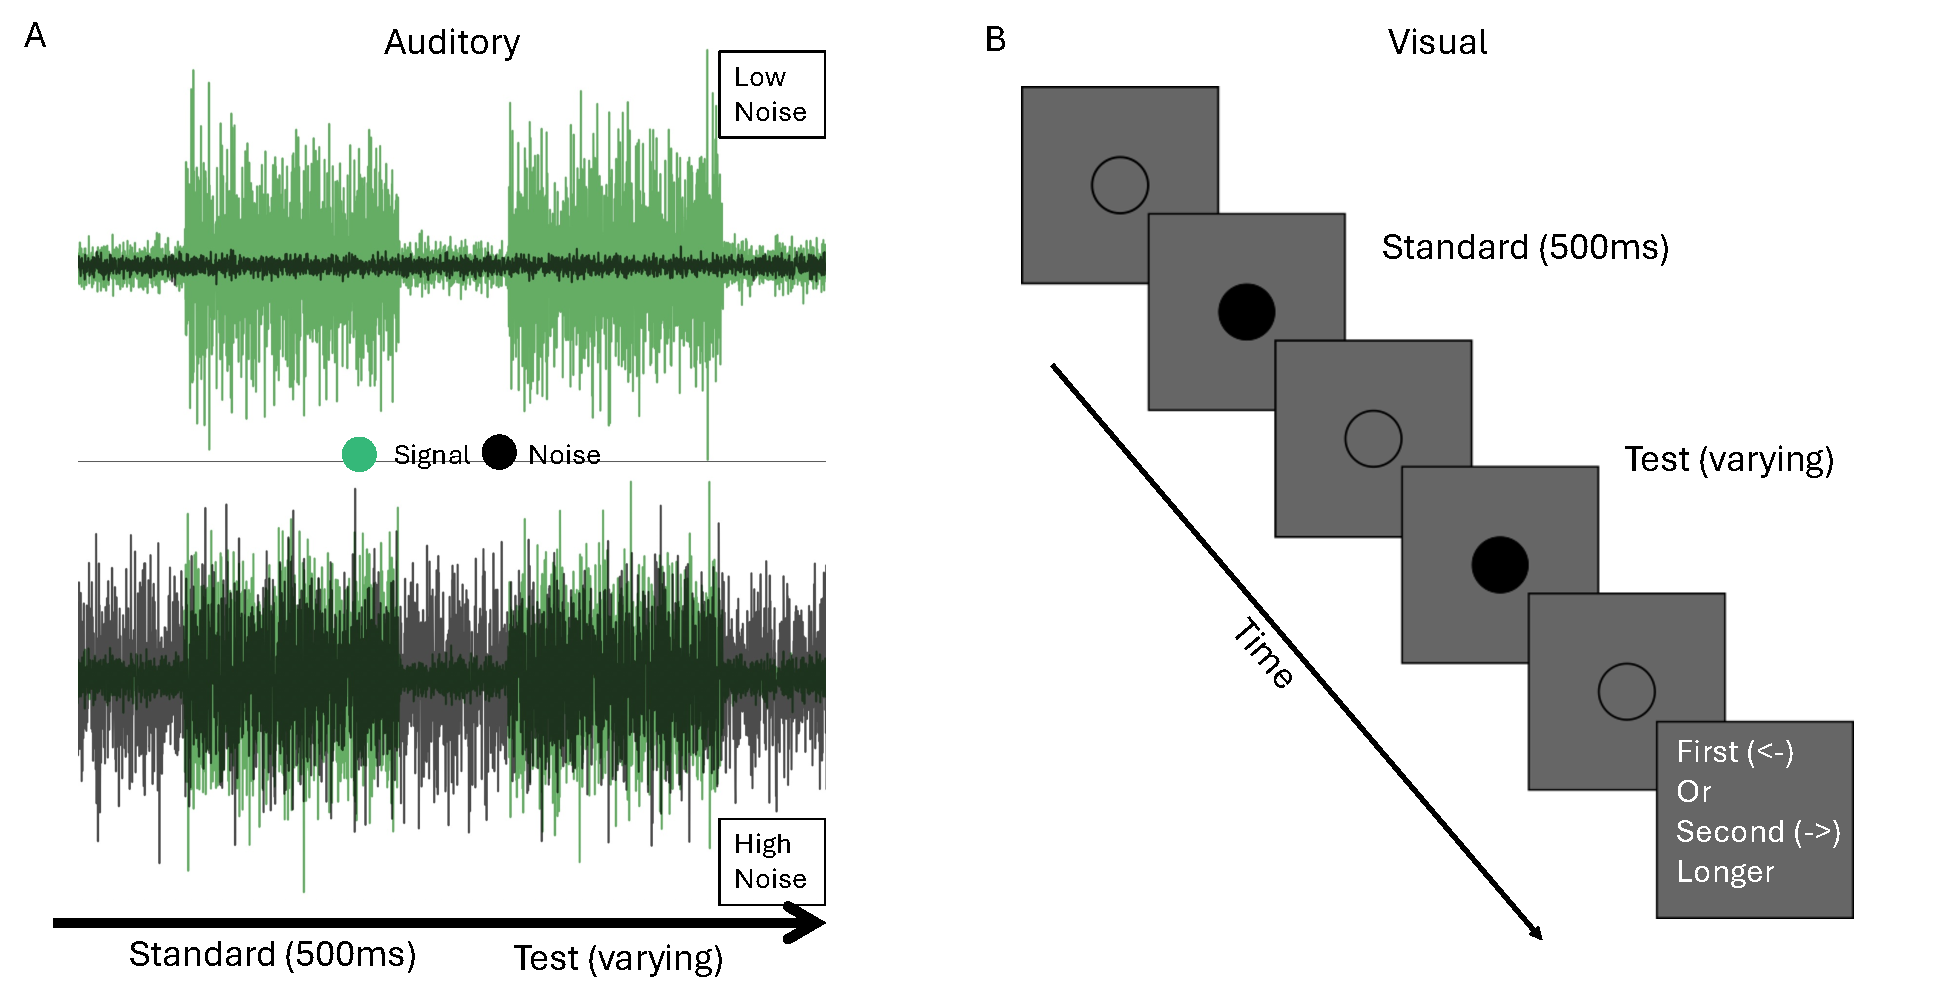
\includegraphics[width=28.360in,height=6.860in,keepaspectratio]{ms_latex/assets/figures/unimodal_tasks_timeline.pdf}};
\path[fill=poster050505, draw=none, rounded corners=0.045in] (1.450,24.900) rectangle (8.970,24.050);
\node[anchor=north west, text width=7.120in, align=left, inner sep=0pt] at (1.680,24.770) {\color{posterffffff}\bfseries \fontsize{0.560in}{0.672in}\selectfont \raggedright \spaceskip=0.32em plus 0.10em minus 0.06em A \textperiodcentered{} UNIMODAL CALIBRATION\par};
\node[anchor=north west, text width=28.600in, align=left, inner sep=0pt] at (1.200,17.600) {\color{poster242424}\fontsize{0.560in}{0.672in}\selectfont \raggedright \spaceskip=0.32em plus 0.10em minus 0.06em Auditory and visual duration-discrimination tasks calibrate per-modality sensory noise.\par};
\path[fill=posterffffff, draw=poster8a8a8a, line width=0.020in, rounded corners=0.045in] (1.200,16.200) rectangle (29.800,9.750);
\node[anchor=north west, inner sep=0pt] at (1.320,16.080) {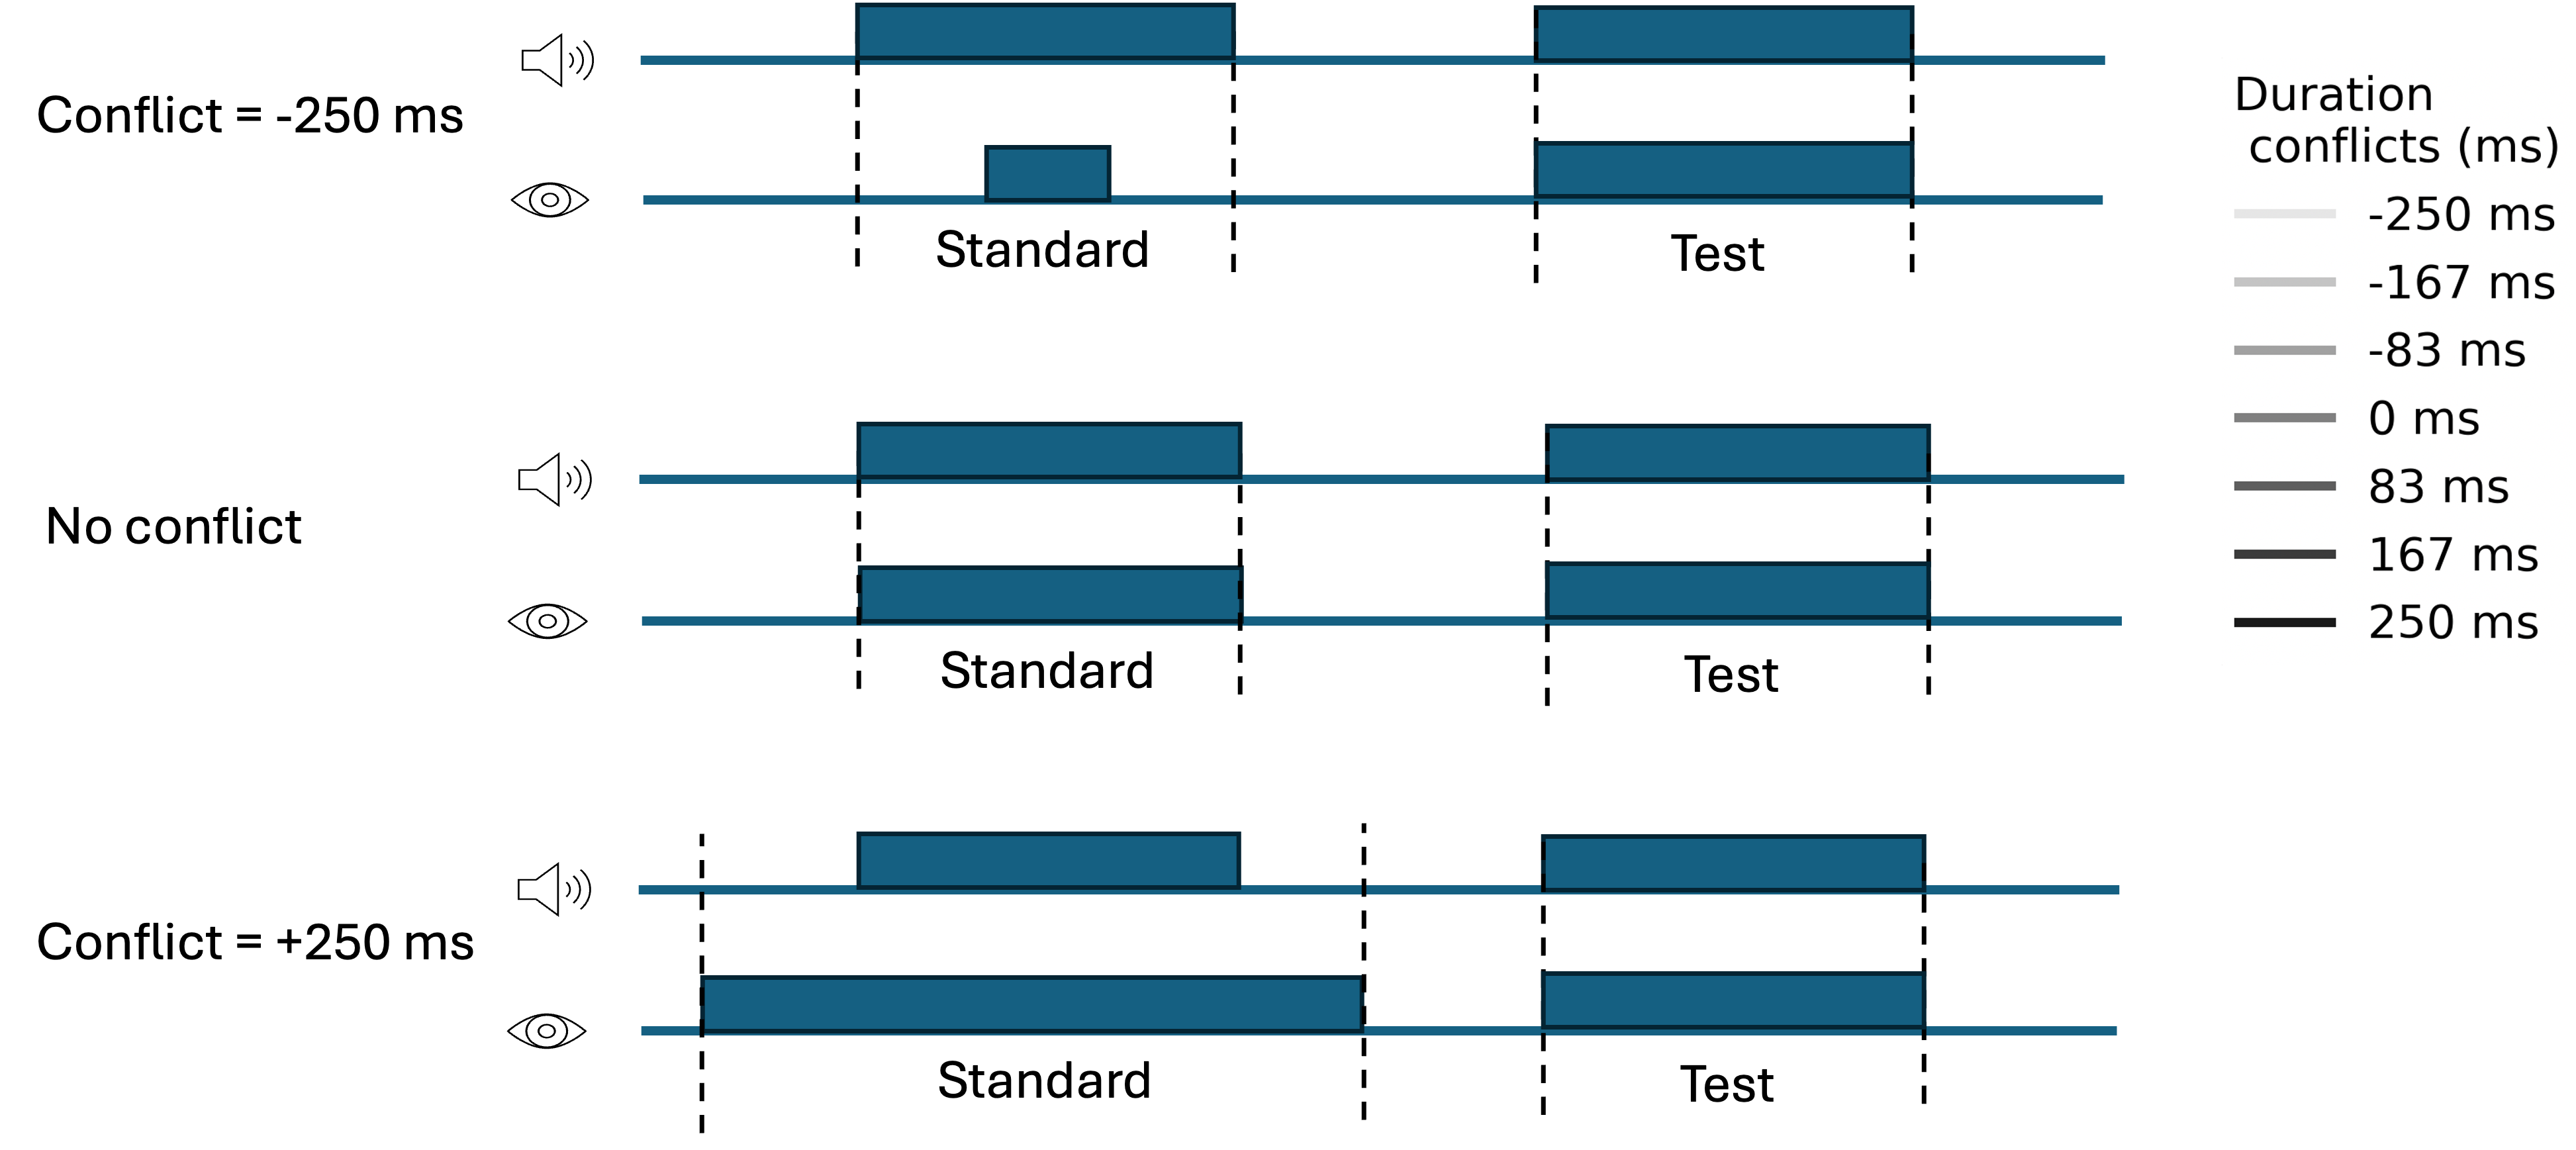
\includegraphics[width=28.360in,height=6.210in,keepaspectratio]{ms_latex/assets/figures/bimodal_exp_scheme.png}};
\path[fill=poster050505, draw=none, rounded corners=0.045in] (1.450,15.950) rectangle (8.690,15.100);
\node[anchor=north west, text width=6.840in, align=left, inner sep=0pt] at (1.680,15.820) {\color{posterffffff}\bfseries \fontsize{0.560in}{0.672in}\selectfont \raggedright \spaceskip=0.32em plus 0.10em minus 0.06em B \textperiodcentered{} BIMODAL AV CONFLICT\par};
\node[anchor=north west, text width=28.600in, align=left, inner sep=0pt] at (1.200,9.300) {\color{poster242424}\fontsize{0.560in}{0.672in}\selectfont \raggedright \spaceskip=0.32em plus 0.10em minus 0.06em Conflict is applied only to the visual standard; observers judge which interval was longer in audition.\par};
\path[fill=posterffffff, draw=poster8a8a8a, line width=0.020in, rounded corners=0.045in] (1.200,5.150) rectangle (8.100,3.400);
\draw[poster050505, line width=0.080in] (1.200,5.150) -- (8.100,5.150);
\node[anchor=north west, text width=6.900in, align=center, inner sep=0pt] at (1.200,4.920) {\color{poster050505}\bfseries \fontsize{0.740in}{0.888in}\selectfont \centering \spaceskip=0.32em plus 0.10em minus 0.06em 7\par};
\node[anchor=north west, text width=6.600in, align=center, inner sep=0pt] at (1.350,4.030) {\color{poster4a4a4a}\fontsize{0.560in}{0.672in}\selectfont \centering \spaceskip=0.32em plus 0.10em minus 0.06em conflicts\par};
\path[fill=posterffffff, draw=poster8a8a8a, line width=0.020in, rounded corners=0.045in] (8.350,5.150) rectangle (15.250,3.400);
\draw[poster050505, line width=0.080in] (8.350,5.150) -- (15.250,5.150);
\node[anchor=north west, text width=6.900in, align=center, inner sep=0pt] at (8.350,4.920) {\color{poster050505}\bfseries \fontsize{0.740in}{0.888in}\selectfont \centering \spaceskip=0.32em plus 0.10em minus 0.06em ±250\par};
\node[anchor=north west, text width=6.600in, align=center, inner sep=0pt] at (8.500,4.030) {\color{poster4a4a4a}\fontsize{0.560in}{0.672in}\selectfont \centering \spaceskip=0.32em plus 0.10em minus 0.06em ms range\par};
\path[fill=posterffffff, draw=poster8a8a8a, line width=0.020in, rounded corners=0.045in] (15.500,5.150) rectangle (22.400,3.400);
\draw[poster050505, line width=0.080in] (15.500,5.150) -- (22.400,5.150);
\node[anchor=north west, text width=6.900in, align=center, inner sep=0pt] at (15.500,4.920) {\color{poster050505}\bfseries \fontsize{0.740in}{0.888in}\selectfont \centering \spaceskip=0.32em plus 0.10em minus 0.06em 2\par};
\node[anchor=north west, text width=6.600in, align=center, inner sep=0pt] at (15.650,4.030) {\color{poster4a4a4a}\fontsize{0.560in}{0.672in}\selectfont \centering \spaceskip=0.32em plus 0.10em minus 0.06em noise levels\par};
\path[fill=posterffffff, draw=poster8a8a8a, line width=0.020in, rounded corners=0.045in] (22.650,5.150) rectangle (29.550,3.400);
\draw[poster050505, line width=0.080in] (22.650,5.150) -- (29.550,5.150);
\node[anchor=north west, text width=6.900in, align=center, inner sep=0pt] at (22.650,4.920) {\color{poster050505}\bfseries \fontsize{0.740in}{0.888in}\selectfont \centering \spaceskip=0.32em plus 0.10em minus 0.06em 2,156\par};
\node[anchor=north west, text width=6.600in, align=center, inner sep=0pt] at (22.800,4.030) {\color{poster4a4a4a}\fontsize{0.560in}{0.672in}\selectfont \centering \spaceskip=0.32em plus 0.10em minus 0.06em trials/subj\par};
\path[fill=poster050505, draw=none, rounded corners=0.045in] (30.700,34.620) rectangle (32.150,33.700);
\node[anchor=north west, text width=1.250in, align=center, inner sep=0pt] at (30.800,34.450) {\color{posterffffff}\bfseries \fontsize{0.580in}{0.696in}\selectfont \centering \spaceskip=0.32em plus 0.10em minus 0.06em 03\par};
\node[anchor=north west, text width=26.800in, align=left, inner sep=0pt] at (32.500,34.520) {\color{poster050505}\bfseries \fontsize{0.860in}{1.032in}\selectfont \raggedright \spaceskip=0.32em plus 0.10em minus 0.06em Cue Reliability\par};
\draw[poster050505, line width=0.055in] (30.700,33.580) -- (59.300,33.580);
\node[anchor=north west, text width=28.600in, align=left, inner sep=0pt] at (30.700,33.040) {\color{poster242424}\fontsize{0.600in}{0.720in}\selectfont \raggedright \spaceskip=0.32em plus 0.10em minus 0.06em Auditory reliability is highest at low noise and lowest at high noise; vision sits in between.\par};
\path[fill=posterffffff, draw=poster8a8a8a, line width=0.020in, rounded corners=0.045in] (30.700,30.650) rectangle (59.300,22.250);
\node[anchor=north west, inner sep=0pt] at (30.820,30.530) {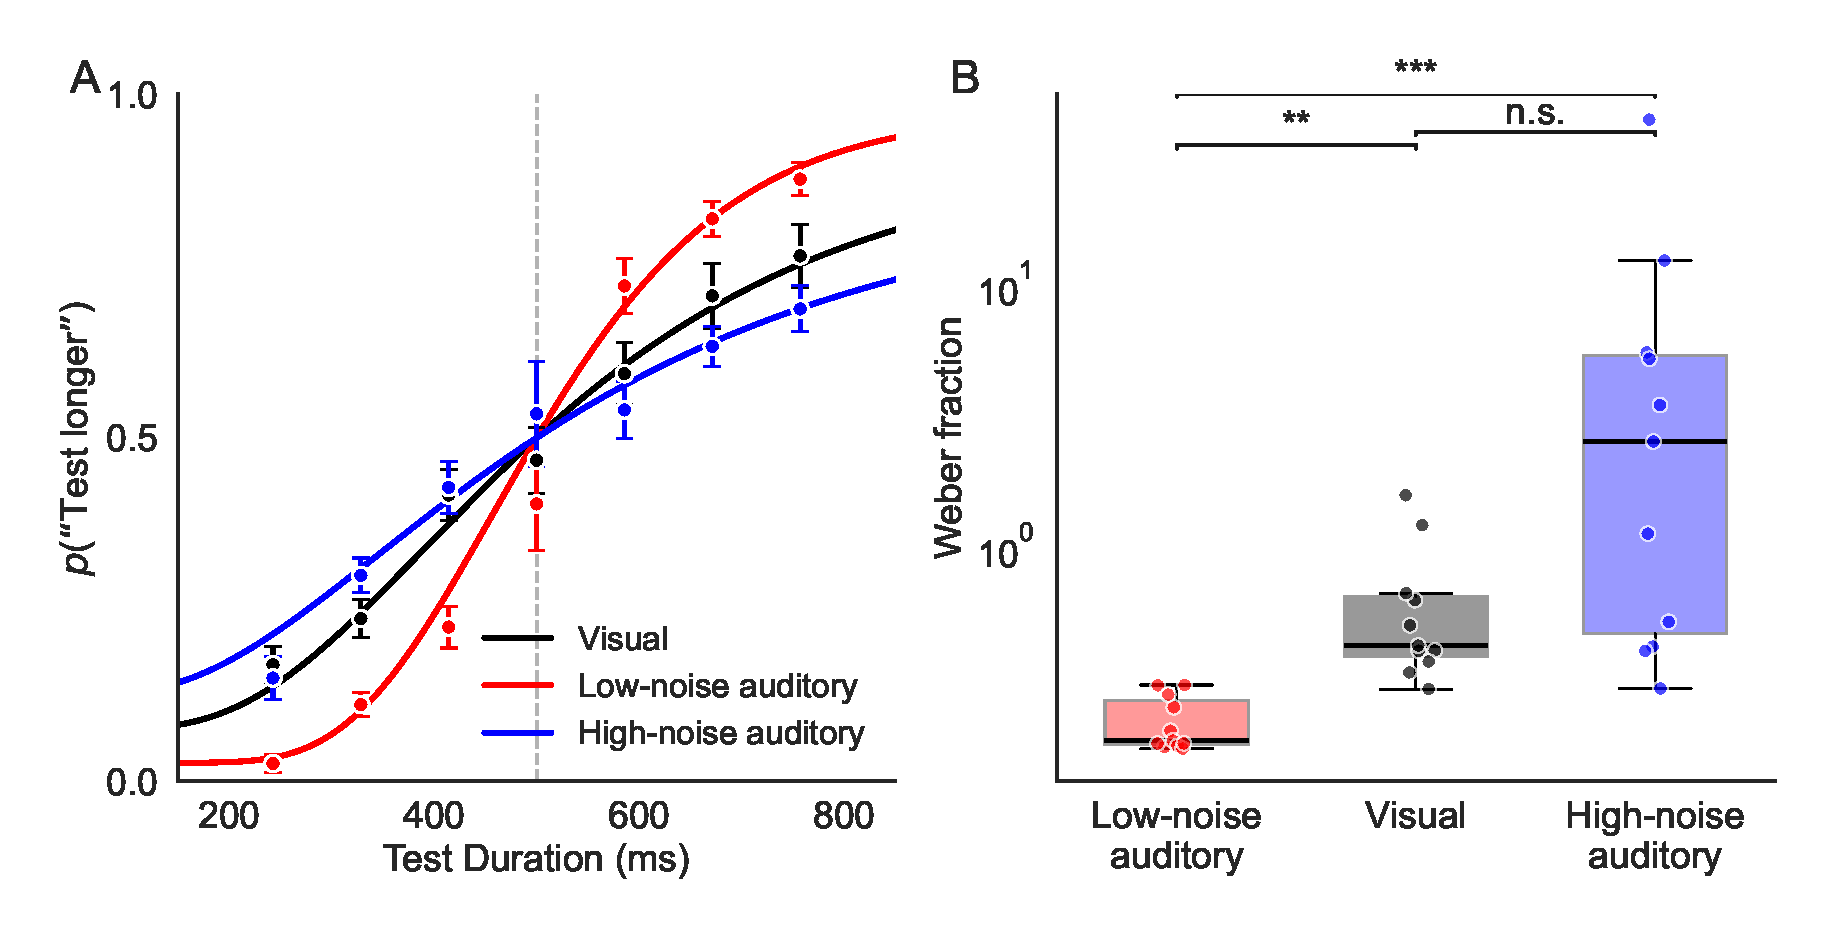
\includegraphics[width=28.360in,height=8.160in,keepaspectratio]{ms_latex/assets/figures/psychometric_curves_publication.pdf}};
\path[fill=posterffffff, draw=poster8a8a8a, line width=0.020in, rounded corners=0.045in] (30.700,21.700) rectangle (39.983,19.950);
\draw[poster050505, line width=0.080in] (30.700,21.700) -- (39.983,21.700);
\node[anchor=north west, text width=9.283in, align=center, inner sep=0pt] at (30.700,21.470) {\color{poster050505}\bfseries \fontsize{0.740in}{0.888in}\selectfont \centering \spaceskip=0.32em plus 0.10em minus 0.06em 0.18\par};
\node[anchor=north west, text width=8.983in, align=center, inner sep=0pt] at (30.850,20.580) {\color{poster4a4a4a}\fontsize{0.560in}{0.672in}\selectfont \centering \spaceskip=0.32em plus 0.10em minus 0.06em WF low-noise\par};
\path[fill=posterffffff, draw=poster8a8a8a, line width=0.020in, rounded corners=0.045in] (40.233,21.700) rectangle (49.517,19.950);
\draw[poster050505, line width=0.080in] (40.233,21.700) -- (49.517,21.700);
\node[anchor=north west, text width=9.283in, align=center, inner sep=0pt] at (40.233,21.470) {\color{poster050505}\bfseries \fontsize{0.740in}{0.888in}\selectfont \centering \spaceskip=0.32em plus 0.10em minus 0.06em 0.42\par};
\node[anchor=north west, text width=8.983in, align=center, inner sep=0pt] at (40.383,20.580) {\color{poster4a4a4a}\fontsize{0.560in}{0.672in}\selectfont \centering \spaceskip=0.32em plus 0.10em minus 0.06em WF visual\par};
\path[fill=posterffffff, draw=poster8a8a8a, line width=0.020in, rounded corners=0.045in] (49.767,21.700) rectangle (59.050,19.950);
\draw[poster050505, line width=0.080in] (49.767,21.700) -- (59.050,21.700);
\node[anchor=north west, text width=9.283in, align=center, inner sep=0pt] at (49.767,21.470) {\color{poster050505}\bfseries \fontsize{0.740in}{0.888in}\selectfont \centering \spaceskip=0.32em plus 0.10em minus 0.06em 2.54\par};
\node[anchor=north west, text width=8.983in, align=center, inner sep=0pt] at (49.917,20.580) {\color{poster4a4a4a}\fontsize{0.560in}{0.672in}\selectfont \centering \spaceskip=0.32em plus 0.10em minus 0.06em WF high-noise\par};
\path[fill=poster050505, draw=none, rounded corners=0.045in] (30.700,19.670) rectangle (32.150,18.750);
\node[anchor=north west, text width=1.250in, align=center, inner sep=0pt] at (30.800,19.500) {\color{posterffffff}\bfseries \fontsize{0.580in}{0.696in}\selectfont \centering \spaceskip=0.32em plus 0.10em minus 0.06em 04\par};
\node[anchor=north west, text width=26.800in, align=left, inner sep=0pt] at (32.500,19.570) {\color{poster050505}\bfseries \fontsize{0.860in}{1.032in}\selectfont \raggedright \spaceskip=0.32em plus 0.10em minus 0.06em Modality Bias\par};
\draw[poster050505, line width=0.055in] (30.700,18.630) -- (59.300,18.630);
\node[anchor=north west, text width=8.200in, align=right, inner sep=0pt] at (51.100,19.430) {\color{poster4a4a4a}\fontsize{0.560in}{0.672in}\selectfont \raggedleft \spaceskip=0.32em plus 0.10em minus 0.06em cross-modal calibration\par};
\node[anchor=north west, text width=28.600in, align=left, inner sep=0pt] at (30.700,18.090) {\color{poster242424}\fontsize{0.560in}{0.672in}\selectfont \raggedright \spaceskip=0.32em plus 0.10em minus 0.06em We estimate each subject's auditory-visual bias before adding conflict, then correct the visual stimulus so nominal zero conflict is perceptually matched.\par};
\path[fill=posterffffff, draw=poster8a8a8a, line width=0.020in, rounded corners=0.045in] (30.700,15.750) rectangle (59.300,7.950);
\node[anchor=north west, inner sep=0pt] at (30.820,15.630) {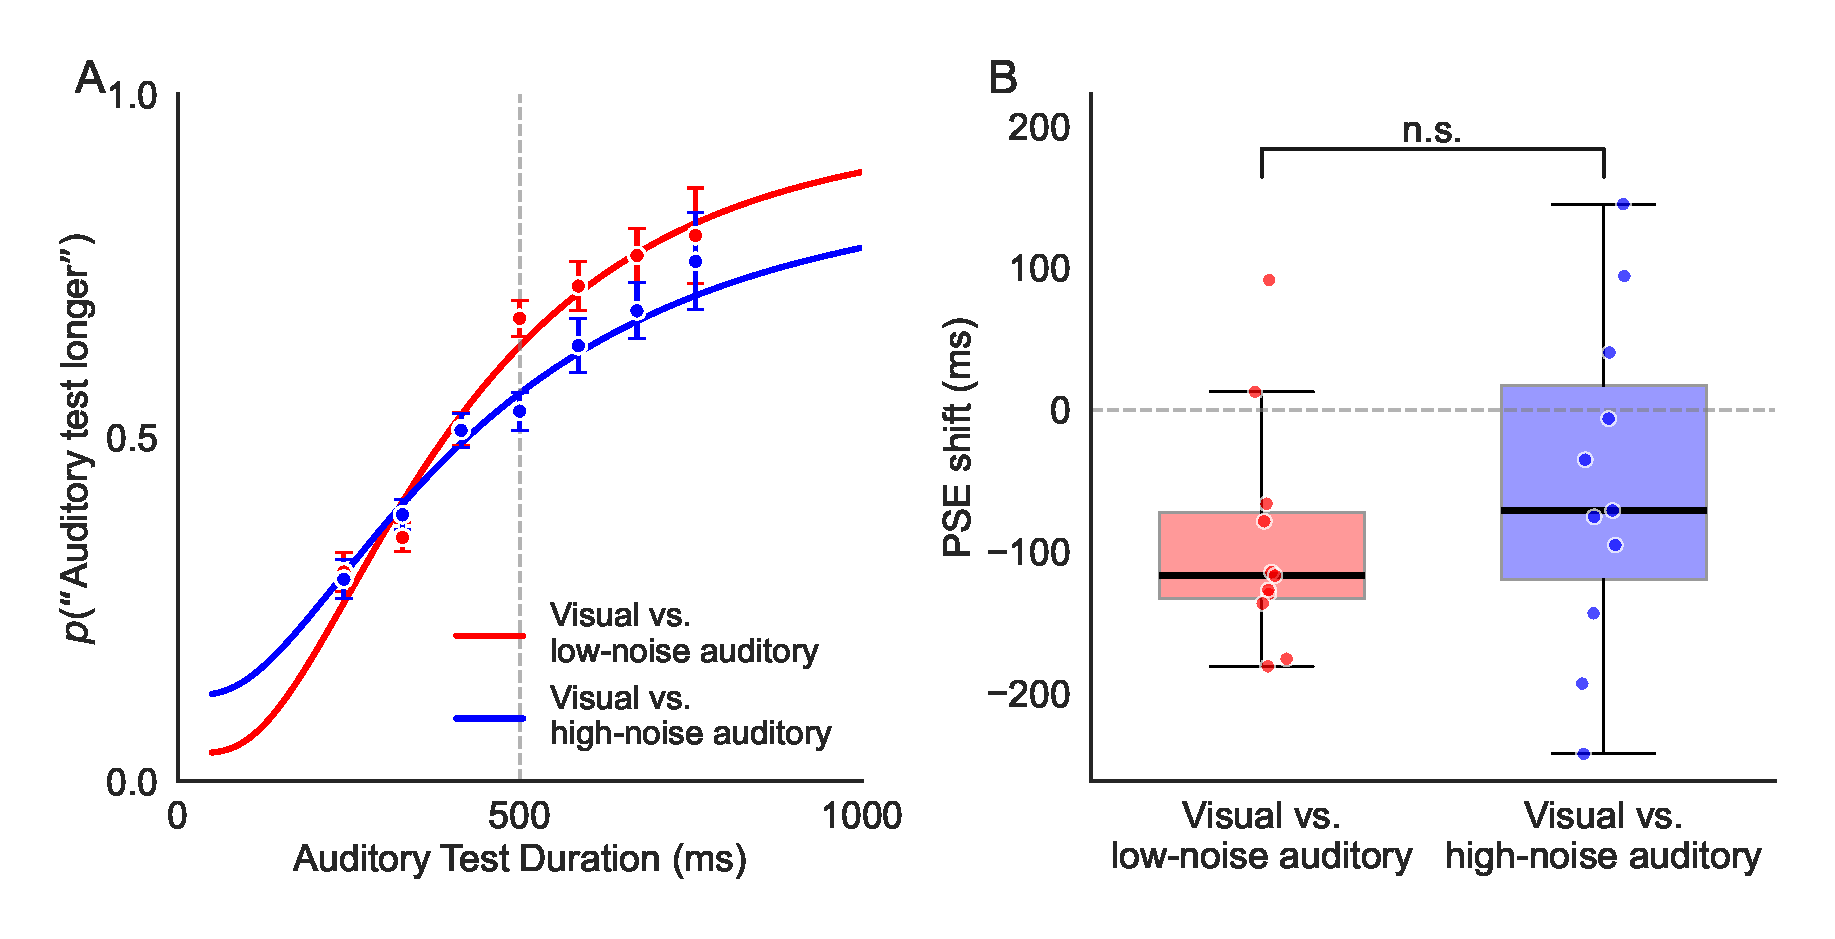
\includegraphics[width=28.360in,height=7.560in,keepaspectratio]{ms_latex/assets/figures/psychometric_curves_crossmodal.pdf}};
\path[fill=posterffffff, draw=poster8a8a8a, line width=0.020in, rounded corners=0.045in] (30.700,7.400) rectangle (44.750,5.350);
\draw[poster050505, line width=0.100in] (30.700,7.400) -- (30.700,5.350);
\node[anchor=north west, text width=13.350in, align=left, inner sep=0pt] at (31.120,7.120) {\color{poster4a4a4a}\bfseries \fontsize{0.560in}{0.672in}\selectfont \raggedright \spaceskip=0.32em plus 0.10em minus 0.06em LOW-NOISE PSE SHIFT\par};
\node[anchor=north west, text width=13.350in, align=left, inner sep=0pt] at (31.120,6.470) {\color{poster050505}\bfseries \fontsize{0.720in}{0.864in}\selectfont \raggedright \spaceskip=0.32em plus 0.10em minus 0.06em -116 ms\par};
\node[anchor=north west, text width=13.350in, align=left, inner sep=0pt] at (31.120,5.820) {\color{poster4a4a4a}\fontsize{0.560in}{0.672in}\selectfont \raggedright \spaceskip=0.32em plus 0.10em minus 0.06em W = 6, p = .014\par};
\path[fill=posterffffff, draw=poster8a8a8a, line width=0.020in, rounded corners=0.045in] (45.250,7.400) rectangle (59.300,5.350);
\draw[poster050505, line width=0.100in] (45.250,7.400) -- (45.250,5.350);
\node[anchor=north west, text width=13.350in, align=left, inner sep=0pt] at (45.670,7.120) {\color{poster4a4a4a}\bfseries \fontsize{0.560in}{0.672in}\selectfont \raggedright \spaceskip=0.32em plus 0.10em minus 0.06em HIGH-NOISE PSE SHIFT\par};
\node[anchor=north west, text width=13.350in, align=left, inner sep=0pt] at (45.670,6.470) {\color{poster050505}\bfseries \fontsize{0.720in}{0.864in}\selectfont \raggedright \spaceskip=0.32em plus 0.10em minus 0.06em -73 ms\par};
\node[anchor=north west, text width=13.350in, align=left, inner sep=0pt] at (45.670,5.820) {\color{poster4a4a4a}\fontsize{0.560in}{0.672in}\selectfont \raggedright \spaceskip=0.32em plus 0.10em minus 0.06em n.s.\par};
\path[fill=poster050505, draw=none, rounded corners=0.045in] (60.200,34.620) rectangle (61.650,33.700);
\node[anchor=north west, text width=1.250in, align=center, inner sep=0pt] at (60.300,34.450) {\color{posterffffff}\bfseries \fontsize{0.580in}{0.696in}\selectfont \centering \spaceskip=0.32em plus 0.10em minus 0.06em 05\par};
\node[anchor=north west, text width=26.800in, align=left, inner sep=0pt] at (62.000,34.520) {\color{poster050505}\bfseries \fontsize{0.860in}{1.032in}\selectfont \raggedright \spaceskip=0.32em plus 0.10em minus 0.06em Main Result \textperiodcentered{} PSE Shifts\par};
\draw[poster050505, line width=0.055in] (60.200,33.580) -- (88.800,33.580);
\node[anchor=north west, text width=28.600in, align=left, inner sep=0pt] at (60.200,33.040) {\color{poster242424}\fontsize{0.600in}{0.720in}\selectfont \raggedright \spaceskip=0.32em plus 0.10em minus 0.06em Visual bias grows approximately linearly with conflict and is much larger under high auditory noise.\par};
\path[fill=posterffffff, draw=poster8a8a8a, line width=0.020in, rounded corners=0.045in] (60.200,30.700) rectangle (88.800,21.900);
\node[anchor=north west, inner sep=0pt] at (60.320,30.580) {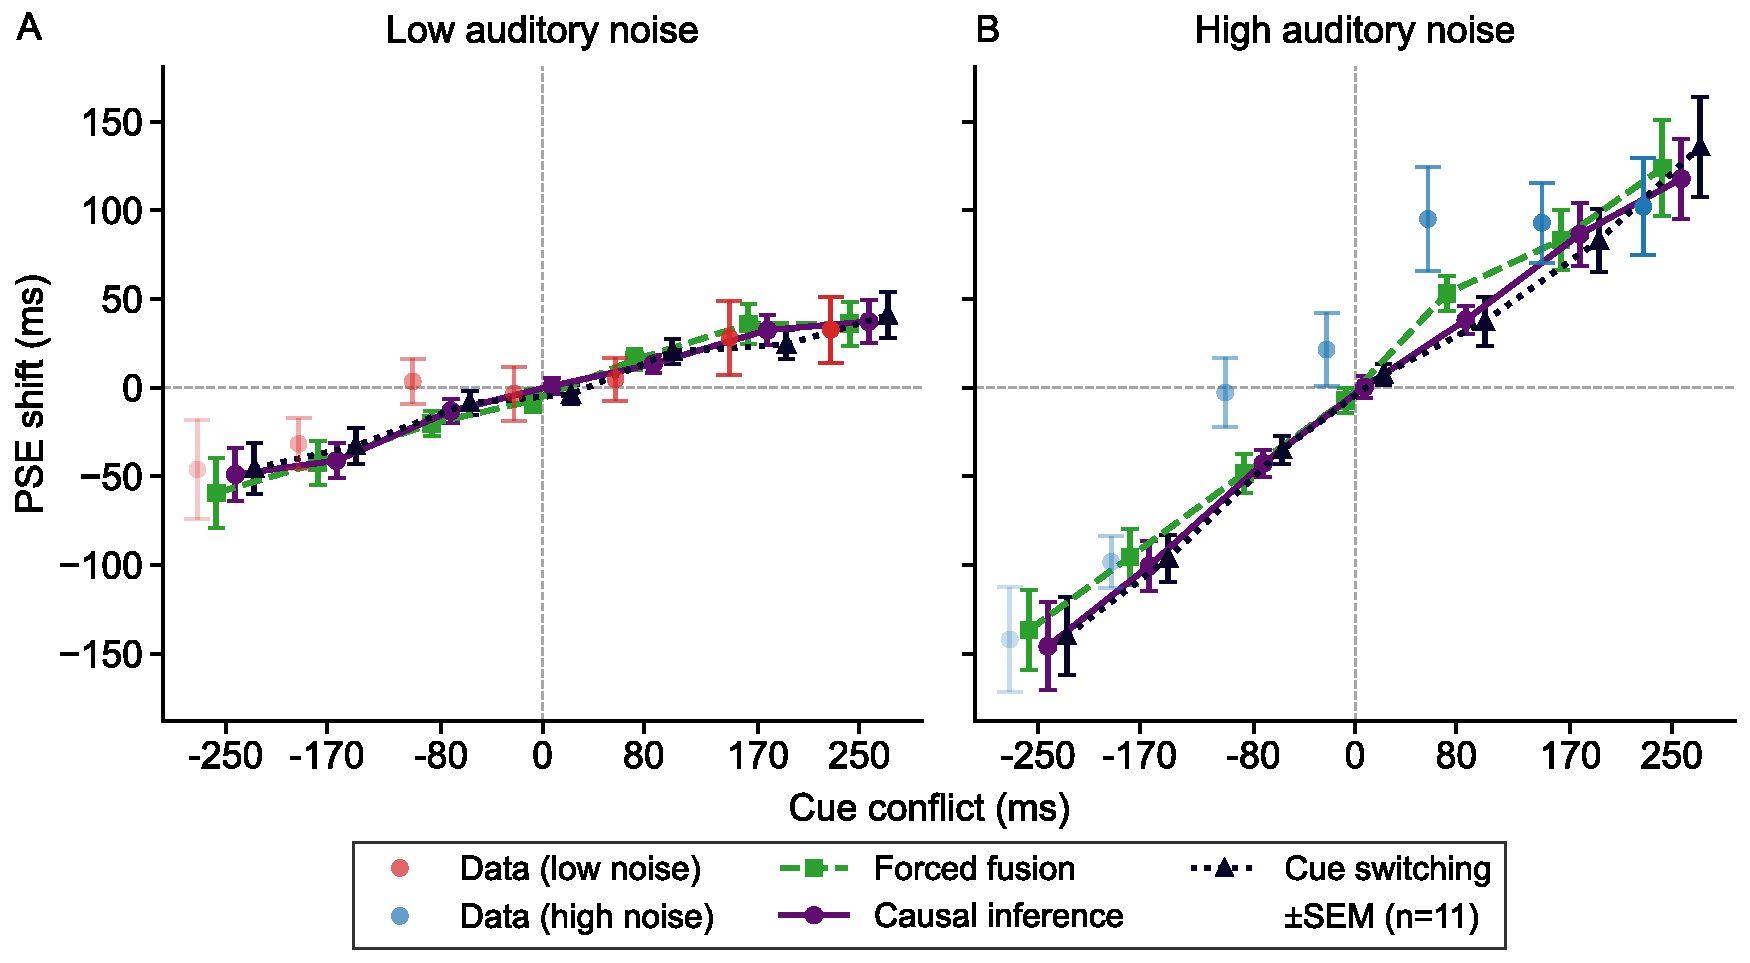
\includegraphics[width=28.360in,height=8.560in,keepaspectratio]{ms_latex/assets/figures/aggregated_mu_vs_models_sem.pdf}};
\path[fill=posterffffff, draw=poster8a8a8a, line width=0.020in, rounded corners=0.045in] (60.200,21.300) rectangle (74.250,19.250);
\draw[poster050505, line width=0.100in] (60.200,21.300) -- (60.200,19.250);
\node[anchor=north west, text width=13.350in, align=left, inner sep=0pt] at (60.620,21.020) {\color{poster4a4a4a}\bfseries \fontsize{0.560in}{0.672in}\selectfont \raggedright \spaceskip=0.32em plus 0.10em minus 0.06em LOW-NOISE SLOPE\par};
\node[anchor=north west, text width=13.350in, align=left, inner sep=0pt] at (60.620,20.370) {\color{poster050505}\bfseries \fontsize{0.720in}{0.864in}\selectfont \raggedright \spaceskip=0.32em plus 0.10em minus 0.06em 0.144\par};
\node[anchor=north west, text width=13.350in, align=left, inner sep=0pt] at (60.620,19.720) {\color{poster4a4a4a}\fontsize{0.560in}{0.672in}\selectfont \raggedright \spaceskip=0.32em plus 0.10em minus 0.06em r = 0.91, p = .004\par};
\path[fill=posterffffff, draw=poster8a8a8a, line width=0.020in, rounded corners=0.045in] (74.750,21.300) rectangle (88.800,19.250);
\draw[poster050505, line width=0.100in] (74.750,21.300) -- (74.750,19.250);
\node[anchor=north west, text width=13.350in, align=left, inner sep=0pt] at (75.170,21.020) {\color{poster4a4a4a}\bfseries \fontsize{0.560in}{0.672in}\selectfont \raggedright \spaceskip=0.32em plus 0.10em minus 0.06em HIGH-NOISE SLOPE\par};
\node[anchor=north west, text width=13.350in, align=left, inner sep=0pt] at (75.170,20.370) {\color{poster050505}\bfseries \fontsize{0.720in}{0.864in}\selectfont \raggedright \spaceskip=0.32em plus 0.10em minus 0.06em 0.606\par};
\node[anchor=north west, text width=13.350in, align=left, inner sep=0pt] at (75.170,19.720) {\color{poster4a4a4a}\fontsize{0.560in}{0.672in}\selectfont \raggedright \spaceskip=0.32em plus 0.10em minus 0.06em r = 0.96, p < .001\par};
\path[fill=poster050505, draw=none, rounded corners=0.045in] (60.200,17.320) rectangle (61.650,16.400);
\node[anchor=north west, text width=1.250in, align=center, inner sep=0pt] at (60.300,17.150) {\color{posterffffff}\bfseries \fontsize{0.580in}{0.696in}\selectfont \centering \spaceskip=0.32em plus 0.10em minus 0.06em 06\par};
\node[anchor=north west, text width=26.800in, align=left, inner sep=0pt] at (62.000,17.220) {\color{poster050505}\bfseries \fontsize{0.860in}{1.032in}\selectfont \raggedright \spaceskip=0.32em plus 0.10em minus 0.06em Models \& Comparison\par};
\draw[poster050505, line width=0.055in] (60.200,16.280) -- (88.800,16.280);
\node[anchor=north west, text width=8.200in, align=right, inner sep=0pt] at (80.600,17.080) {\color{poster4a4a4a}\fontsize{0.560in}{0.672in}\selectfont \raggedleft \spaceskip=0.32em plus 0.10em minus 0.06em free sensory noise\par};
\path[fill=posterffffff, draw=poster8a8a8a, line width=0.020in, rounded corners=0.045in] (60.200,15.850) rectangle (88.800,9.700);
\node[anchor=north west, inner sep=0pt] at (60.320,15.730) {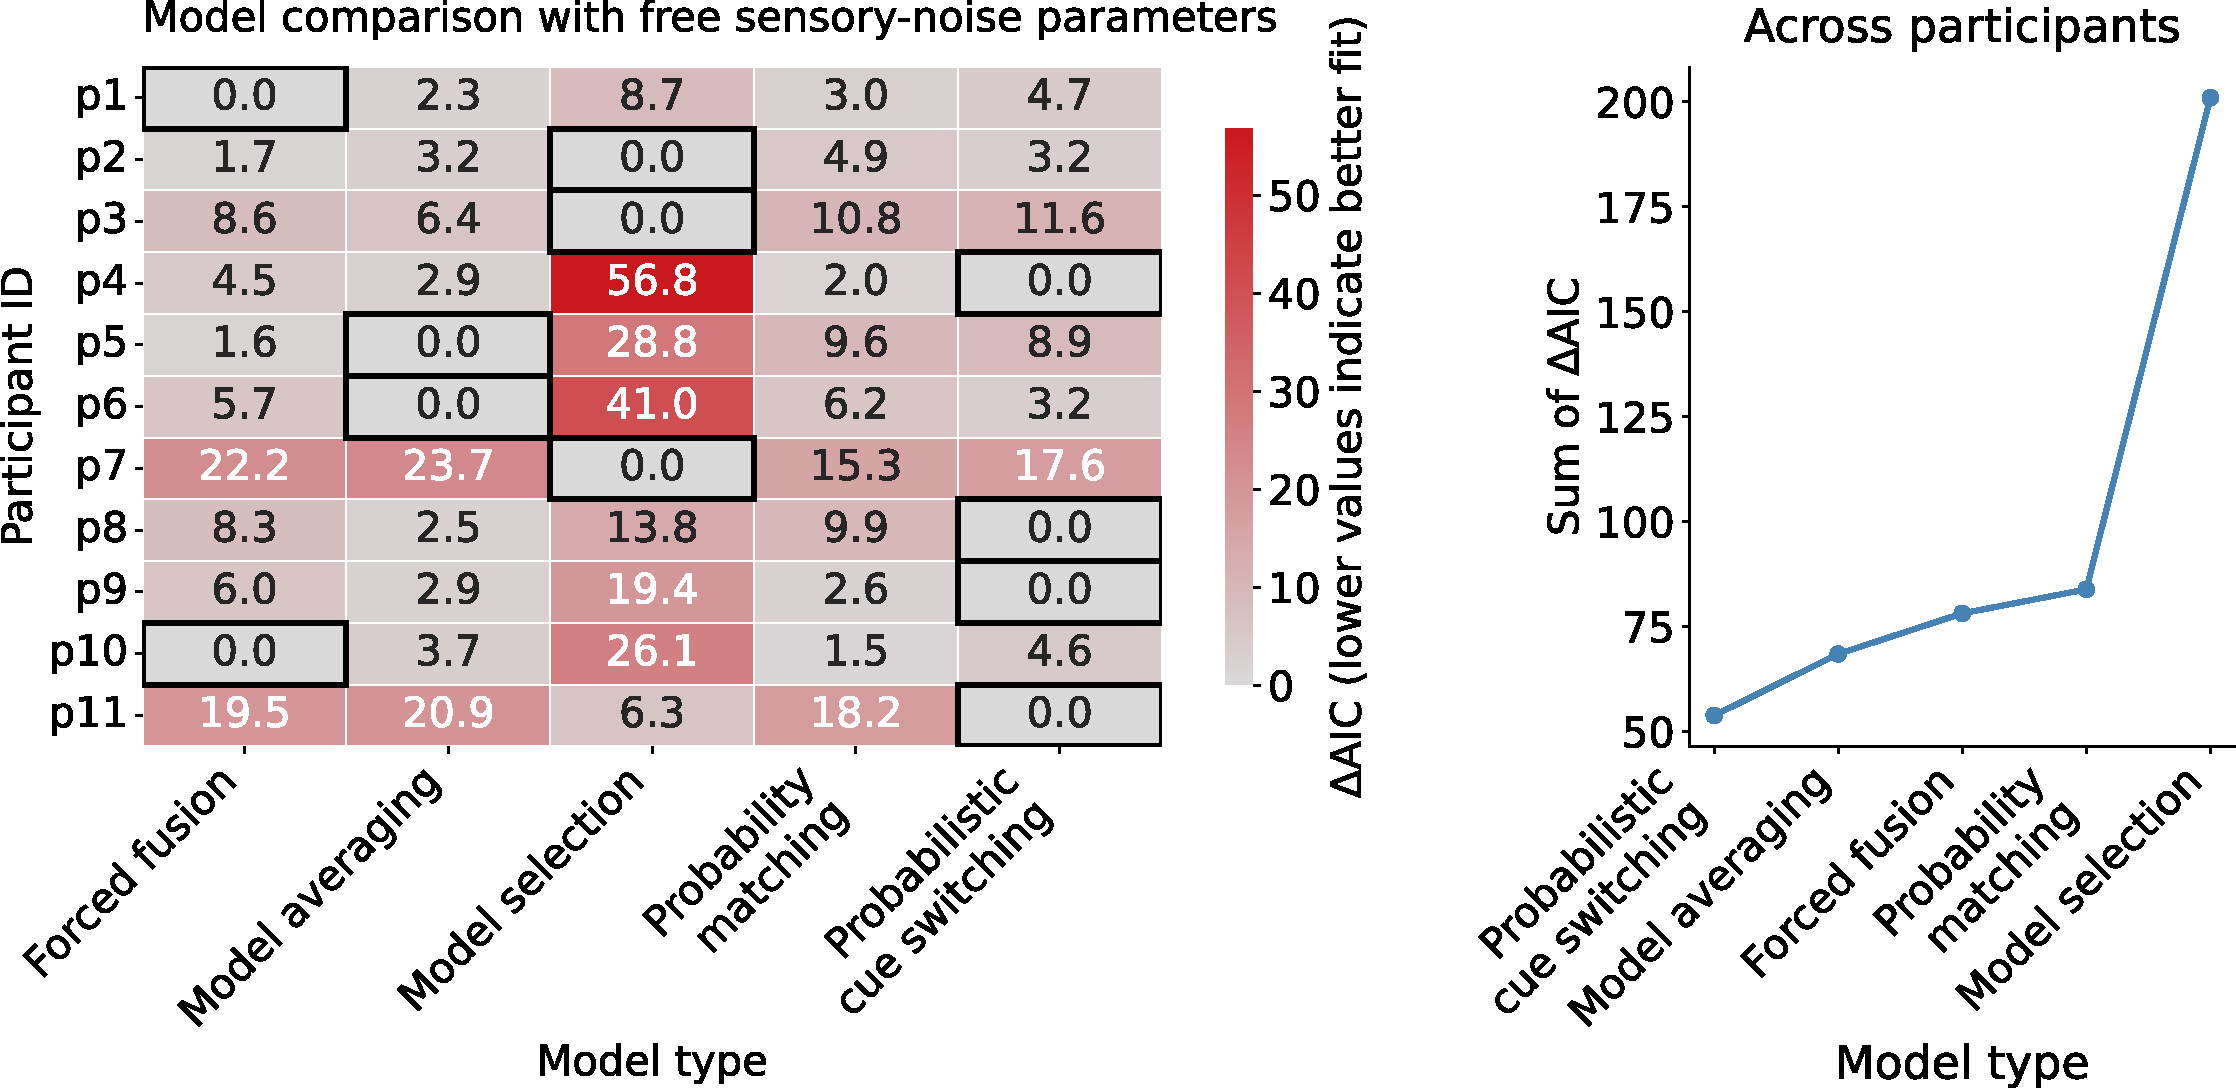
\includegraphics[width=28.360in,height=5.910in,keepaspectratio]{ms_latex/assets/figures/modelCompFree.pdf}};
\path[fill=posterffffff, draw=poster8a8a8a, line width=0.020in, rounded corners=0.045in] (60.200,9.050) rectangle (88.800,6.950);
\draw[poster050505, line width=0.100in] (60.200,9.050) -- (60.200,6.950);
\path[fill=poster050505, draw=none, rounded corners=0.045in] (60.550,8.770) rectangle (61.730,8.050);
\node[anchor=north west, text width=1.180in, align=center, inner sep=0pt] at (60.550,8.660) {\color{posterffffff}\bfseries \fontsize{0.560in}{0.672in}\selectfont \centering \spaceskip=0.32em plus 0.10em minus 0.06em M1\par};
\node[anchor=north west, text width=26.450in, align=left, inner sep=0pt] at (62.050,8.730) {\color{poster050505}\bfseries \fontsize{0.620in}{0.744in}\selectfont \raggedright \spaceskip=0.32em plus 0.10em minus 0.06em Forced fusion\par};
\node[anchor=north west, text width=27.900in, align=left, inner sep=0pt] at (60.550,7.750) {\color{poster242424}\fontsize{0.560in}{0.672in}\selectfont \raggedright \spaceskip=0.32em plus 0.10em minus 0.06em Always integrate auditory and visual cues using reliability-weighted averaging.\par};
\path[fill=posterffffff, draw=poster8a8a8a, line width=0.020in, rounded corners=0.045in] (60.200,6.650) rectangle (88.800,4.550);
\draw[poster050505, line width=0.100in] (60.200,6.650) -- (60.200,4.550);
\path[fill=poster050505, draw=none, rounded corners=0.045in] (60.550,6.370) rectangle (61.730,5.650);
\node[anchor=north west, text width=1.180in, align=center, inner sep=0pt] at (60.550,6.260) {\color{posterffffff}\bfseries \fontsize{0.560in}{0.672in}\selectfont \centering \spaceskip=0.32em plus 0.10em minus 0.06em M2-4\par};
\node[anchor=north west, text width=26.450in, align=left, inner sep=0pt] at (62.050,6.330) {\color{poster050505}\bfseries \fontsize{0.620in}{0.744in}\selectfont \raggedright \spaceskip=0.32em plus 0.10em minus 0.06em Causal inference\par};
\node[anchor=north west, text width=27.900in, align=left, inner sep=0pt] at (60.550,5.350) {\color{poster242424}\fontsize{0.560in}{0.672in}\selectfont \raggedright \spaceskip=0.32em plus 0.10em minus 0.06em Fuse or segregate according to the posterior probability of a common cause.\par};
\path[fill=posterffffff, draw=poster8a8a8a, line width=0.020in, rounded corners=0.045in] (60.200,4.250) rectangle (88.800,2.150);
\draw[poster050505, line width=0.100in] (60.200,4.250) -- (60.200,2.150);
\path[fill=poster050505, draw=none, rounded corners=0.045in] (60.550,3.970) rectangle (61.730,3.250);
\node[anchor=north west, text width=1.180in, align=center, inner sep=0pt] at (60.550,3.860) {\color{posterffffff}\bfseries \fontsize{0.560in}{0.672in}\selectfont \centering \spaceskip=0.32em plus 0.10em minus 0.06em M5\par};
\node[anchor=north west, text width=26.450in, align=left, inner sep=0pt] at (62.050,3.930) {\color{poster050505}\bfseries \fontsize{0.620in}{0.744in}\selectfont \raggedright \spaceskip=0.32em plus 0.10em minus 0.06em Probabilistic cue switching\par};
\node[anchor=north west, text width=27.900in, align=left, inner sep=0pt] at (60.550,2.950) {\color{poster242424}\fontsize{0.560in}{0.672in}\selectfont \raggedright \spaceskip=0.32em plus 0.10em minus 0.06em Use auditory or visual cue alone on each trial with a fixed switching probability.\par};
\path[fill=poster050505, draw=none, rounded corners=0.045in] (60.200,1.800) rectangle (88.800,0.350);
\node[anchor=north west, text width=27.500in, align=left, inner sep=0pt] at (60.750,1.380) {\color{posterffffff}\bfseries \fontsize{0.580in}{0.696in}\selectfont \raggedright \spaceskip=0.32em plus 0.10em minus 0.06em Take-home: linear bias, flat model evidence, and an identifiability limit.\par};
\end{tikzpicture}
\end{document}